\documentclass[
	classe=$2^{de}$,
	landscape,
	twocolumn,
]{évaluation}

\usepackage{tikz-repère}
\usetikzlibrary{calc}

\setlength{\columnsep}{1cm}

\begin{document}

\date{17 mars 2023}

\title{Interrogation : coordonnées de vecteurs\\ (sujet A)}
\maketitle

\begin{exercice}\

	\begin{center}
		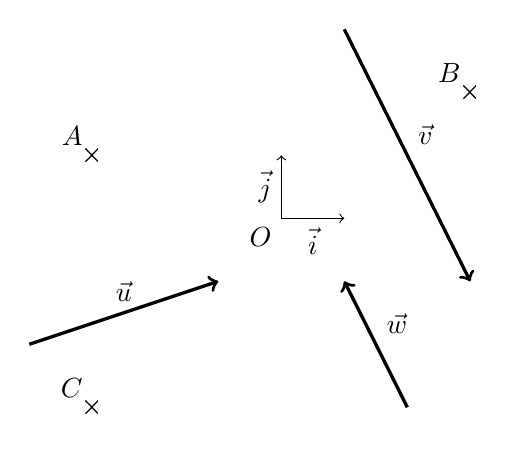
\begin{tikzpicture}[scale=0.8]
			\tikzRepere{-4.5}{4.5}{-3.5}{3.5}[][]
			\node[below left] at (0,0) {$O$};
			\draw[->] (0,0) -- node[below] {$\vec{i}$} (1,0);
			\draw[->] (0,0) -- node[left] {$\vec{j}$} (0,1);

			\node (A) at (-3,1) {×};
			\node (B) at (3,2) {×};
			\node (C) at (-3,-3) {×};
			\foreach \p in {A,B,C} {
					\node[above left] at (\p) {$\p$};
				}
			\coordinate (U) at (3,1);
			\coordinate (V) at (2,-4);
			\coordinate (W) at (-1,2);

			\draw[->,very thick] (-4,-2) -- node[above] {$\vec{u}$} ++(U);
			\draw[->,very thick] (1,3) -- node[above right] {$\vec{v}$} ++(V);
			\draw[->,very thick] (2,-3) -- node[above right] {$\vec{w}$} ++(W);

			\ifdefined\makeCorrection
				\node[red] (D) at ($(A) + (U)$) {×};
				\node[red] (E) at ($(B) + 0.5*(V)$) {×};
				\node[red] (F) at ($(C) + (U) + (W)$) {×};
				\foreach \p in {D,E,F} {
						\node[red,above left] at (\p) {$\p$};
					}
			\fi
		\end{tikzpicture}
	\end{center}
	Placer ci-dessus les points $D$, $E$ et $F$ tels que :
	\begin{multicols}{3}
		\begin{enumerate}
			\item $\vec{AD} = \vec{u}$
			\item $\vec{BE} = \dfrac{1}{2}\vec{v}$
			\item $\vec{CF} = \vec{u} + \vec{w}$
		\end{enumerate}
	\end{multicols}
\end{exercice}

\begin{exercice}\
	On donne les vecteur $\vec{u} \begin{pmatrix}2 \\ -3\end{pmatrix}$ et $\vec{v} \begin{pmatrix}x \\ y\end{pmatrix}$, où $a$ et $b$ sont des nombres réels.

	Déterminer la valeur de $x$ et de $y$ dans les cas suivants, en détaillant :
	\begin{enumerate}
		\setlength{\itemsep}{1.5em}
		\item $4\vec{u} - 3\vec{v} = 0$
		\item $\dfrac{3}{4}\vec{u} = -\dfrac{7}{5}\vec{v}$
	\end{enumerate}
\end{exercice}

%=================================================
%================== SUJET B ======================
%=================================================
\setcounter{exercice}{1}
\newpage

\title{Interrogation : coordonnées de vecteurs\\ (sujet B)}
\maketitle

\begin{exercice}\

	\begin{center}
		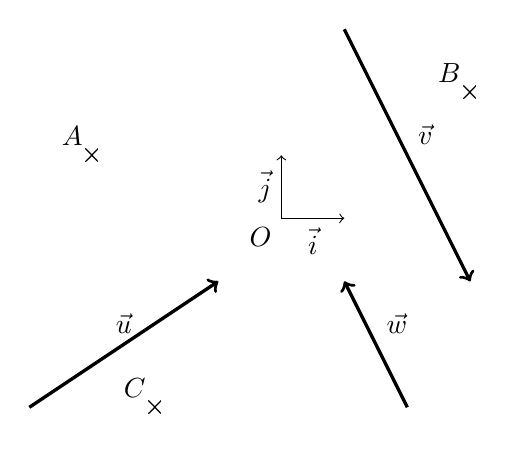
\begin{tikzpicture}[scale=0.8]
			\tikzRepere{-4.5}{4.5}{-3.5}{3.5}[][]
			\node[below left] at (0,0) {$O$};
			\draw[->] (0,0) -- node[below] {$\vec{i}$} (1,0);
			\draw[->] (0,0) -- node[left] {$\vec{j}$} (0,1);

			\node (A) at (-3,1) {×};
			\node (B) at (3,2) {×};
			\node (C) at (-2,-3) {×};
			\foreach \p in {A,B,C} {
					\node[above left] at (\p) {$\p$};
				}
			\coordinate (U) at (3,2);
			\coordinate (V) at (2,-4);
			\coordinate (W) at (-1,2);

			\draw[->,very thick] (-4,-3) -- node[above] {$\vec{u}$} ++(U);
			\draw[->,very thick] (1,3) -- node[above right] {$\vec{v}$} ++(V);
			\draw[->,very thick] (2,-3) -- node[above right] {$\vec{w}$} ++(W);

			\ifdefined\makeCorrection
				\node[red] (D) at ($(A) + (U)$) {×};
				\node[red] (E) at ($(B) + 0.5*(V)$) {×};
				\node[red] (F) at ($(C) + (U) + (W)$) {×};
				\foreach \p in {D,E,F} {
						\node[red,above left] at (\p) {$\p$};
					}
			\fi
		\end{tikzpicture}
	\end{center}
	Placer ci-dessus les points $D$, $E$ et $F$ tels que :
	\begin{multicols}{3}
		\begin{enumerate}
			\item $\vec{AD} = \vec{u}$
			\item $\vec{BE} = \dfrac{1}{2}\vec{v}$
			\item $\vec{CF} = \vec{u} + \vec{w}$
		\end{enumerate}
	\end{multicols}
\end{exercice}

\begin{exercice}\
	On donne les vecteur $\vec{u} \begin{pmatrix}3 \\ -2\end{pmatrix}$ et $\vec{v} \begin{pmatrix}x \\ y\end{pmatrix}$, où $a$ et $b$ sont des nombres réels.

	Déterminer la valeur de $x$ et de $y$ dans les cas suivants :
	\begin{enumerate}
		\setlength{\itemsep}{1.5em}
		\item $6\vec{u} - 5\vec{v} = 0$
		\item $\dfrac{5}{4}\vec{u} = -\dfrac{3}{5}\vec{v}$
	\end{enumerate}
\end{exercice}

\end{document}